\begin{thesischapter}
    \section{绪论}
    本章为sauthss模板的使用示例文档,对本模板的使用时的常见用法和常见问题进行解释和说明。
    \subsection{模板相关}
    本模板是沈阳航空航天大学本科毕设\LaTeX 模板,旨在简化毕业论文写作过程中的格式调整过程。内容与排版部分参考沈阳航空航天大学自动化学院2024年本科毕业设计模板制作并修改。本模板适合有一定编程基础或\LaTeX 写作经验的同学使用。\par
    毕设基本信息在main.tex头部定义,在使用此模板前,请自行按照注释修改相关变量。\par
    \begin{Verbatim}
    % --------------- 基本信息配置区--------------- 
    % 将此处替换为你的中文标题,需要换行处用\\隔开
    \newcommand{\getTitle}{{沈阳航空航天大学毕业设计(本科)\\Latex模板}}
    % 将此处替换为你的英文标题,需要换行处用\\隔开
    \newcommand{\getTitleEn}
    {{SAU Thesis Latex Template for Undergraduate}}
    % 将此处替换为你的中文关键词,词和词用;隔开
    \newcommand{\getKeywords}{{Latex;沈阳航空航天大学;深度学习}}
    % 将此处替换为你的英文关键词,词和词用;隔开
    \newcommand{\getKeywordsEn}{{Latex;SAU;Deep Learning}}
    % 将此处替换为你的姓名
    \newcommand{\getAuthorName}{{李田所}}
    % 将此处替换为你的学院
    \newcommand{\getInstituteName}{{自动化学院}}
    % 将此处替换为你的专业
    \newcommand{\getMajorName}{{自动化}}
    % 将此处替换为你的班级
    \newcommand{\getClassName}{{自动化2001班}}
    % 将此处替换为你的学号
    \newcommand{\getID}{{20341919810}}
    % 将此处替换为你的指导老师
    \newcommand{\getMentorName}{{张三}}
    % 将此处替换为你的负责教师
    \newcommand{\getSupervisiorName}{{王五}}
    % 是否在首页放置教师签名png,true为放置
    \newcommand{\needMentorsign}{false}
    % 答辩年份
    \newcommand{\getYY}{2024}
    % 答辩月份
    \newcommand{\getMM}{6}
    \end{Verbatim}
    \subsection{已知问题}
    本模板当前存在以下主要问题:
    \begin{itemize}
        \item 页面以浮动体(图片、表格)结束时,可能为下一页新的subsection或subsubsection引入多余空行,请调整文本内容与位置尽量避免此情况。\par
        \item 非技术因素分析部分表格布局与Word版表格布局存在一定出入。\par
    \end{itemize}\par
    若您在使用中遇到其他问题,请在github仓库提交Issue或者向此电子邮箱guhao0521@gmail.com发送电子邮件描述您的问题,以便于我们及时解决。您也可以修改代码自行解决问题并向本仓库提交PR,为本项目做出贡献。\par
    \subsection{摘要部分}
    摘要需要在\textbackslash begin\{thesisabstractcn\}和\textbackslash begin\{thesisabstracten\}环境中进行编写。概述毕业设计的目的,采用的软硬件设计方案或研究方法、步骤等,突出创新点;最终的调试或仿真结果,以及分析得到的研究结论。论文设计方案或者采用方法的优点。
    \subsection{目录部分}
    参考本科毕业设计模板制作,分隔点与模板略有出入,不影响实际使用。“目录”二字用三号字、黑体,居中书写,“目”与“录”之间空两格并加粗。一级目录采用四号宋体;二级目录向右缩进 2 字符,采用小四号宋体;三级目录向右缩进 4 字符采用小四号宋体;英文字母和数字都采用 Times New Roman格式;行间距 22 磅(调整\textbackslash cftbeforesecskip得到,实际测量与word行距相同)。
    \subsection{正文部分}
    本模板与word模板相同,采用三级标题形式划分文章。完成内容时请注意标点符号全半角统一,完成一个段落后使用\textbackslash par来结束段落。\par
    下面为标准章节示例代码:\par
    \begin{Verbatim}
    \begin{thesischapter}%开始章节环境
    \section{绪论}%定义章节名称
    % 一些内容
    % ......
    \subsection{研究背景}%二级标题
    % 一些内容
    % ......
    \subsection{国内外研究现状}%二级标题
    \subsubsection{国内研究现状}%三级标题
    % 一些内容
    % ......
    \subsubsection{国外研究现状}%三级标题
    % 一些内容
    % ......
    \end{thesischapter}%结束章节环境
    \end{Verbatim}
    \subsection{图表示例}
    \subsubsection{表格使用示例}
    \begin{table}[h]
        \centering
        \songti\zihao{5}
        \caption{表格示例}
        \begin{tabular}{ccc}
            \toprule
            依赖名称 & 版本需求 & 安装方式 \\
            \midrule
            Ubuntu & 20.04 LTS & 镜像安装 \\
            ROS2 & Foxy & apt安装 \\
            Pytorch & 2.1.0 & pip安装 \\
            CUDA & 12.2 & sh安装 \\
            QT & 5.15 & apt安装 \\
            ifxradarsdk & 3.5.0 & whl安装 \\
            \bottomrule
        \end{tabular}
        \label{tab:sample}
    \end{table}
    毕业设计模板要求表格均使用三线表,表序和表名均位于表格的上方,在Latex中三线表可依赖宏包booktabs实现,使用\textbackslash toprule,
\textbackslash midrule,\textbackslash bottomrule来控制三线。效果如表\ref{tab:sample}所示。 
    \subsubsection{图片使用示例}
     毕业设计模板要求图片题注需位于在图像下方。如图\ref{fig:sample_1}所示。单张图片使用\textbackslash begin\{figure\}环境,若使用Overleaf可直接将图片拖入浏览器以上传图片。注意所有图片均应存储于Figure文件夹下以便于管理。\par
    \begin{figure}[hb]
        \centering
        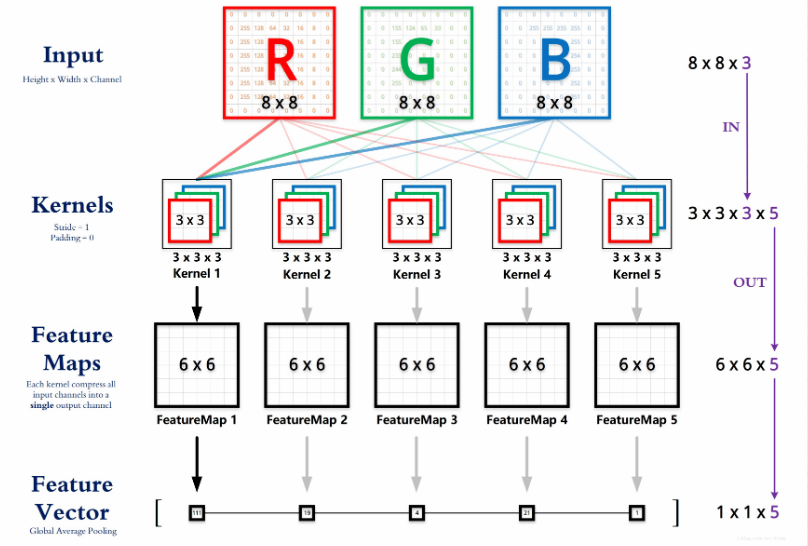
\includegraphics[width=0.4\linewidth]{Figure/sample_1.png}
        \caption{图片样例1}
        \label{fig:sample_1}
    \end{figure}
    当使用多张图片时,可使用subfigure进行插入多张图片。若需引用子图,可以使用\textbackslash subref\{子图label\}进行引用。
    \begin{figure}[h]
        \centering
        \subfigure[常规模块]
        {
            \centering
            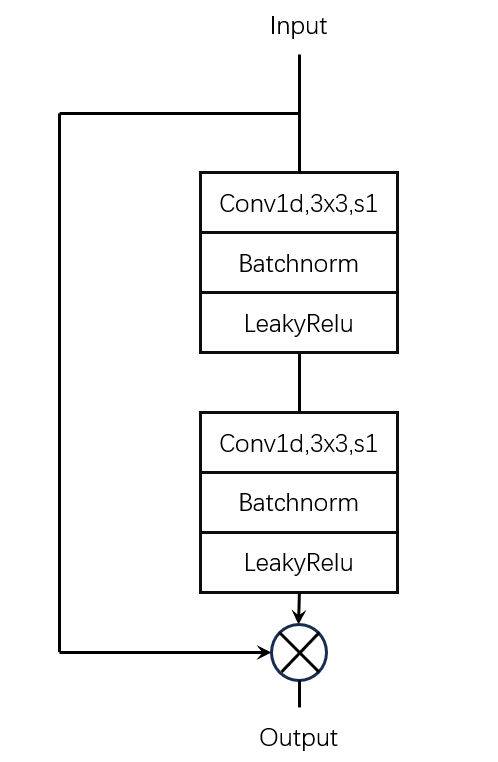
\includegraphics[width=0.44\linewidth]{Figure/resnet1d_flow_a.png}
            \label{fig:resnet1d_flow.a}
        }
        \hfill
        \subfigure[下采样模块]
        {
            \centering
            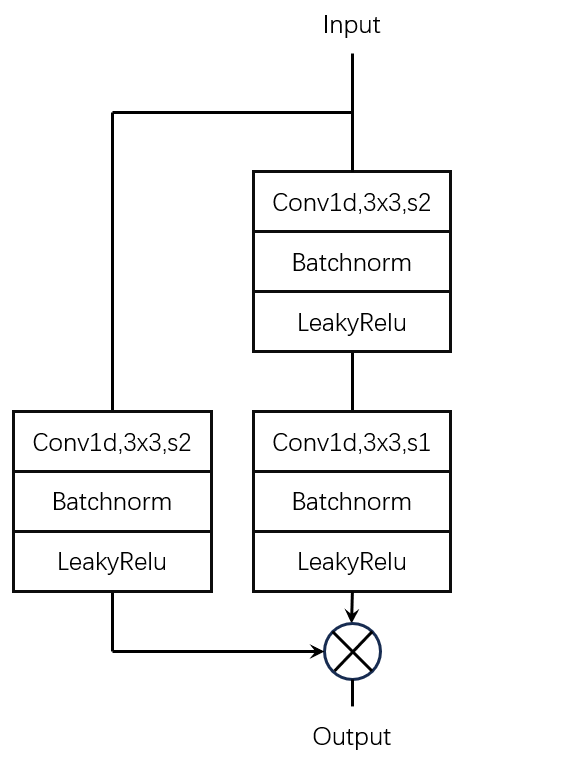
\includegraphics[width=0.52\linewidth]{Figure/resnet1d_flow_b.png}
            \label{fig:resnet1d_flow.b}
        }
        \caption{多张图片示例}
    \end{figure}
    \subsection{公式}
    公式使用\textbackslash begin\{equation\}环境插入,使用通用\LaTeX{}规范即可,如式\ref{eq:mae}。
    \begin{equation}
        MAE = \frac{1}{n} \sum_{i=1}^n |\hat{y}_i - y_i |
        \label{eq:mae}
    \end{equation}\par
    
    \subsection{参考文献}
    参考文献使用GB/T 7714格式进行引用,使用gb7714-2015bibstyle 进行管理,具体引用命令与日常使用类似,\verb|\cite{}|,\verb|\citet{}|,\verb|\citeauthor{}|具体用法见相应文档\cite{hushidong_biblatex-gb7714-2015}。\par
    例如\verb|\cite{feng2018wing}|=\cite{feng2018wing},... 相对于的 bib 文件的书写基本上直接用 Google Scholar 拷贝的 BibTex 即可,部分属性按提示进行微调。\par

    \subsection{版权声明}
    本模板参考Homework in Chinese\cite{overleaf2024homework}模板修改而来。使用文档参考北大本科非官方模板\cite{pku_undergrad_thesis_template}进行编写。\par
    本示例文档和模板遵循 LATEX Project Public License 和 Attribution 4.0 International (CC BY 4.0) 开源协议。
\end{thesischapter}